\documentclass{article}
\usepackage[utf8]{inputenc}
\usepackage{authblk}
\usepackage{setspace}
\usepackage[margin=1.25in]{geometry}
\usepackage{graphicx}
\usepackage{xcolor}
\usepackage{float}
\graphicspath{ {./figures/} }
\usepackage{amsmath,amssymb,amsfonts}
\usepackage{booktabs}
\usepackage{natbib}
\usepackage{hyperref}
\hypersetup{colorlinks=true, linkcolor=blue, citecolor=blue, urlcolor=blue}

\title{\textbf{Does High-Yield Credit Lead Equities? Relative Bond Performance and Next-Week Stock Returns}}
\author[1]{SIQuant Research}
\affil[1]{Hypothesis $\times$ Quant}
\date{\today}
\onehalfspacing

\begin{document}
\maketitle

\begin{abstract}
\noindent \textbf{Hypothesis:} $H_0$: the five-day relative return of high-yield versus Treasury bonds does not predict the next five-day SPY return; $H_1$: the relation is positive \\
\textbf{Data:} 2,504 daily observations of HYG, IEF and SPY, 2016-10-31 to 2026-10-16 \\
\textbf{Method:} OLS with Newey--West HAC errors (10 lags) and a 2,000-draw circular-shift placebo; the decision needs both one-sided $p<0.05$ \\
\textbf{Results:} $\beta=-0.0761$ (HAC $t=-0.53$, $p=0.7030$; placebo $p=0.6462$), $R^2=0.0018$. \\
\textbf{Research decision:} \colorbox[rgb]{0.75,0.15,0.15}{\textcolor{white}{\textbf{\,REJECTED\,}}}
\end{abstract}

\section{Design}
Credit markets are often argued to price risk earlier than equities \citep{gilchrist2012credit}. The predictor is observed at the close of day $t$ and the outcome covers days $t+1$ to $t+5$. Total-return ETFs are used because they are free and liquid; they embed duration, so the Treasury leg is a duration-adjusted benchmark rather than a pure credit spread.

\section{Results}
\begin{figure}[H]
\centering
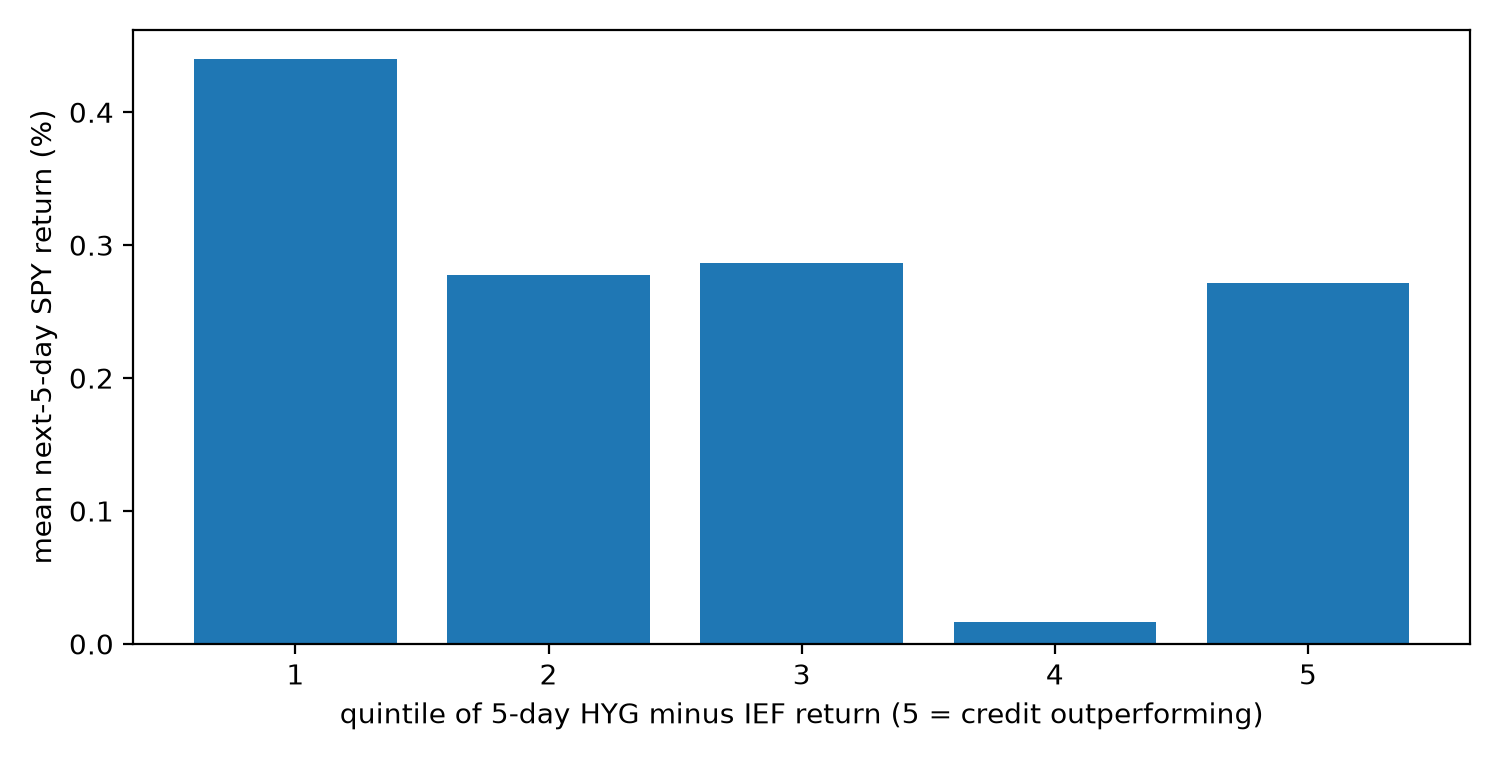
\includegraphics[width=0.8\textwidth]{fig1_credit_quintile_spy.png}
\caption{Mean next-week SPY return by quintile of the credit signal.}
\end{figure}

Adding SPY's own trailing five-day return as a control gives a coefficient of -0.0665 ($t=-0.39$) on the credit signal.

\section{Limitations}
HYG and IEF differ in duration, so the signal also reflects interest-rate moves. The overlap of five-day windows reduces the effective sample size. Daily closes of ETFs and the index are not perfectly synchronous.


\bibliographystyle{plainnat}
\bibliography{references}

\end{document}
